\documentclass[twoside]{article}

\usepackage{subfigure, graphicx}
\usepackage{listings}
\usepackage{syntax}
\usepackage[grid]{multicol}
\usepackage{listings, color}


\lstset{frame=tb,
  language=Java,
  aboveskip=3mm,
  belowskip=3mm,
  showstringspaces=false,
  columns=flexible,
  basicstyle={\small\ttfamily},
  numbers=none,
  numberstyle=\tiny\color{gray},
  keywordstyle=\color{blue},
  commentstyle=\color{dkgreen},
  stringstyle=\color{mauve},
  breaklines=true,
  breakatwhitespace=true,
  tabsize=3
}
\input{packs.tex}

%------------------------------------------------------------------------------
%	TITLE SECTION
%------------------------------------------------------------------------------
\title{\vspace{-15mm}\fontsize{24pt}{10pt}\selectfont\textbf{
    Synthesising a Compiler} } % Article title

\author{
  \large
  \textsc{Josh Reese}\\[2mm] % Your name
  \normalsize \href{mailto:jreese@cs.umd.edu}{jreese@cs.umd.edu}
  \vspace{-5mm}
}
\date{}

%------------------------------------------------------------------------------

\begin{document}
\maketitle % Insert title
\thispagestyle{fancy} % All pages have headers and footers

%------------------------------------------------------------------------------
%	ABSTRACT
%------------------------------------------------------------------------------
%% \begin{abstract}
%% \noindent \lipsum[1] % Dummy abstract text
%% \end{abstract}

%------------------------------------------------------------------------------
%	ARTICLE CONTENTS
%------------------------------------------------------------------------------
%% \begin{multicols}{2} % Two-column layout throughout the main article text

%------------------------------------------------------------------------------
% Motivation
%------------------------------------------------------------------------------
\section{Motivation}
Reasoning about the functionality and properties of modern programming
languages is a challenging and arduous task. However, in order to make any
sense of programs it must be the case that the languages used
can be analysed. One way to reduce the difficulty of reasoning about a
language is to reduce the language itself to a much simpler core
language. Examples of attempts to formalise Javascript can be found in
\cite{ljs,js}. Having this core language with
well defined semantics makes it much easier to reason about the
semantics of a more complicated, but related, language. However,
translating from one language to a simpler core is no trivial task.

Recent work in program synthesis shows very interesting results for
generating code that is able to fulfil previously defined
specifications \cite{flash,invert,sygus,feedback,sketch}. In this work
we will leverage the ideas from program synthesis to automatically
generate code to translate from the more complex, feature-rich
language (which will call language $F$), to the simpler core
language (language $S$). To accomplish this we will use specifications
of the two languages and test inputs written in language $F$ to
synthesise a compiler from language $F$ to language $S$.

%-----------------------------------------------------------------------------
% INTRO
%------------------------------------------------------------------------------
\section{Summary}
It is the main goal of this work to automatically generate code that
compiles programs written in some language, $F$, to some other
language, $S$, where $S \subset F$. To do this we have implemented two
separate languages in Rascal, interpreters for each, and a
synthesiser, also in Rascal. This synthesiser takes, as input,
programs written in language $F$ and produces code which will
translate programs in language $F$ to programs in language $S$.

\subsection{Rascal}
Rascal is a metaprogramming language being developed primarily by the
SWAT group at Centrum Wiskunde and Informatica in Amsterdam
\cite{rascal}. The motivation behind Rascal is to provide a single
tool for effectively analysing, transforming and generating source
code. Since Rascal integrates many aspects of code generation and
program analysis into 
one language it is a natural choice for a project of this
nature. Rascal also provides a very clean way to specify a concrete
syntax and abstract syntax for a language, will automatically generate
a parser for this language, and exports a simple interface for
transforming a concrete syntax tree (CST) into an abstract syntax tree
(AST). For example if one has specified a grammar called \texttt{Prog},
all that needs to be done to generate an AST for this grammar is:
\begin{lstlisting}
public Prog parse(loc l) = parse(#Prog, l);
public Prog load(loc l)  = implode(#Prog, parse(l));
\end{lstlisting}
In this example both the \texttt{parse(\#Prog, l)} and
\texttt{implode(\#Prog, parse(l))} functions are built-in functions
inside Rascal which will generate a CST and AST, respectively. 

In addition to the features previously mentioned Rascal includes
built-in features specifically for tree traversal and manipulation
with the \texttt{visit} concept. This concept allows for automated
traversal of a tree-like structure where each node is visited and
operations can be performed on each node. These operations can include
some form of side effect as well as modifying or replacing the current
element, among others \cite{rascalvisit}.

%------------------------------------------------------------------------------
% Solution
%------------------------------------------------------------------------------
\section{Solution}
In order to accomplish the goals of this project we first had to
design and implement two languages one containing syntactic sugar, and
one core sugar-free language. Once these languages were constructed we
then had to develop interpreters for each in order to verify that the
results of the programs we were generating were indeed correct. After
the interpreters for both languages were finished we developed a
compiler that would translate programs in language $F$ to programs in
language
$S$. The reason for this was to have some frame of reference as to
what the final synthesised compiler should look like and how it should
behave. Finally, once all of this was complete, we were able to begin
development on the synthesiser that would automatically produce the
code for compiling from language $F$ to language $S$.

\subsection{Languages $F$ and $S$}
As previously mentioned we developed two languages for this
project. These two languages are extremely similar with only three key
differences: language $F$ allows for multiple bindings in a let
expression, multiple parameters to a function and the addition of
\texttt{else if} condition to the standard \texttt{if then else}. In
addition to this, each language contains standard arithmetic operations
(i.e. addition, subtraction, etc), standard comparators (less than,
greater that, etc), function applications, and sequencing of
expressions. A program in either language is made up of a number of
global lets followed by an expression. Grammars for these languages
can be found in Figure \ref{fig:grammars}.
\begin{figure}[h]
  \begin{minipage}[t]{0.5\linewidth}
    \centering
    \begin{grammar}
      <Prog> ::= <Letg>* ';;' <Exp> 

      <Letg> ::= 'let' '(' {<Ident> ','}* ')' '=' '(' {<Exp> ','}* ')' 'end' 

      <Elif> ::= 'else if' <Exp> 'then' <Exp> 

      <Exp>  ::= <Ident>
      \alt <Natural> 
      \alt '(' <Exp> ')' 
      \alt 'let' '(' {<Ident> ','}* ')' '=' '(' {<Exp> ','}* ')' 'in' <Exp> 'end' 
      \alt 'if' <Exp> 'then' <Exp> <Elif>* 'else' <Exp> 'end' 
      \alt 'fun' '(' {<Ident> ','}* ')' '->' <Exp>
      \alt <Exp> '*' <Exp> 
      \alt <Exp> '/' <Exp> 
      \alt <Exp> '\%' <Exp> 
      \alt <Exp> '+' <Exp> 
      \alt <Exp> '-' <Exp> 
      \alt <Exp> '=' <Exp> 
      \alt <Exp> '>' <Exp> 
      \alt <Exp> '<' <Exp> 
      \alt <Exp> '>=' <Exp> 
      \alt <Exp> '<=' <Exp>
      \alt <Ident> '(' {<Exp> ','}* ')' 
      \alt <Exp> ';' <Exp>
    \end{grammar}
  \end{minipage}
  \hspace{0.5cm} \vline \hspace{0.5cm} 
  \begin{minipage}[t]{0.45\linewidth}
    \begin{grammar}
      <Prog> ::= <Letg>* ';;' <Exp> 

      <Letg> ::= 'let' '(' {<Ident> ','}* ')' '=' '(' {<Exp> ','}* ')' 'end' 

      <Exp>  ::= <Ident>
      \alt <Natural> 
      \alt '(' <Exp> ')' 
      \alt 'let' <Ident> '=' <Exp> 'in' <Exp> 'end' 
      \alt 'if' <Exp> 'then' <Exp> 'else' <Exp> 'end' 
      \alt 'fun' <Ident> '->' <Exp>
      \alt <Exp> '*' <Exp> 
      \alt <Exp> '/' <Exp> 
      \alt <Exp> '\%' <Exp> 
      \alt <Exp> '+' <Exp> 
      \alt <Exp> '-' <Exp> 
      \alt <Exp> '=' <Exp> 
      \alt <Exp> '>' <Exp> 
      \alt <Exp> '<' <Exp> 
      \alt <Exp> '>=' <Exp> 
      \alt <Exp> '<=' <Exp>
      \alt <Ident> '(' {<Exp> ','}* ')' 
      \alt <Exp> ';' <Exp>
    \end{grammar}
  \end{minipage}
  \caption{Grammars for languages F and S.}
  \label{fig:grammars}
\end{figure}
Both of these languages were constructed in Rascal along with
interpreters for each. 

\subsection{Compiler}
There are two convenient aspects of Rascal that make the compiler
between these two languages somewhat formulaic: function overloading
and patterns as formal parameters. Function overloading works in the
standard fashion of multiple functions which have the same name and
only differ in the parameters. However, Rascal has the ability to use
patterns as formal parameters which lets the programmer match
different constructors to the same type as opposed to just different
type. With these features the compiler, written in Rascal, and using
Rascal's function overloading and pattern parameters is somewhat
formulaic. For example consider the following code, used to compile
addition in language $F$ to addition in language $S$:
\begin{lstlisting}
public lang::DFunc::AST::Exp comp(add(Exp e1, Exp e2)) = add(comp(e1),comp(e2));
\end{lstlisting}
Here we see a function, \texttt{comp()}, which takes, as a parameter, a
pattern which matches the \texttt{add} node in language $F$ and
returns an \texttt{add} node in language $S$ with each component of
the \texttt{add} node compiled into a language $S$ node. This a
simple example since \texttt{add} nodes in language $F$ are structured
identically to \texttt{add} nodes in language $S$. A more complicated
example takes function nodes, \texttt{func}, in language $F$ and
converts them to \texttt{func} nodes in language $S$. The code for
this follows:
\begin{lstlisting}
public lang::DFunc::AST::Exp comp(func([str f], Exp body)) = func(f,comp(body));
public lang::DFunc::AST::Exp comp(func([str f0, *str fn], Exp body)) =
             func(f0,comp(func(fn,body)));
\end{lstlisting}
Once again we leverage the pattern matching capabilities in Rascal to
not only match the function call on a \texttt{func} node but also
match the structure of that node. The function in the first line will
only be executed when called with a \texttt{func} node from language
$F$ that has one formal parameter. It will then return a \texttt{func}
node from language $S$ with the body compiled into a language $S$
node. The next two lines show the recursive case which will be called
when a \texttt{func} node from language $F$ has multiple
parameters. This case will create a language $S$ \texttt{func} node
with the first parameter from the language $F$ \texttt{func} node and
recursively call the \texttt{comp} function on a new language $F$
\texttt{func} node which contains a list of the remaining parameters
and the body of the original function. The cases for \texttt{let} and
\texttt{else if} follow similar logic.

\subsection{Synthesiser}
It is the goal of the synthesiser to take input programs and generate
the code for the compiler described in the previous section. A
pictorial representation of how the synthesiser should work can be
found in Figure \ref{fig:synth}. The synthesiser works in two stages:
reading input and code generation. As input the synthesiser will take
programs written in language $F$, convert it to its corresponding AST,
and use the structure of the AST to synthesise code which transforms
programs of that style to programs in language $S$. In order to
accomplish this we use Rascal's \texttt{visit} concept to traverse the
language $F$ tree and perform certain operations based on the
structure of that node. Building off the previous example of compiling
\texttt{add} nodes from language $F$ to \texttt{add} nodes of language
$S$ we can give the synthesiser the following program:

\lstset{language=ML}
\begin{lstlisting}
;;
x+x
\end{lstlisting}
From this program we will generate the following AST:
\texttt{add(exp(var(x)),exp(var(x)))}. When the synthesiser analyses
the \texttt{add} node, it will notice that this is a node which
contains two parts \texttt{exp()} and \texttt{exp()} and is called
\texttt{add}. This will be used to help generate the parameters to
this node's \texttt{comp} function and the type of node to convert to
in order to make this a valid node in language $S$. Since there are
two parts to this node, it will take a node called \texttt{add} which
is comprised of two parameters. Next, the synthesiser will examine
each part of the \texttt{add} node and use the type to generate the
types that make up the \texttt{add} parameter and the types that make
up the return value. Since both of these are of type \texttt{exp} the
synthesiser will insert \texttt{Exp e1} and \texttt{Exp e2} as the
parts of the \texttt{add} node in the parameter. Since each sub part
of a language $F$ node needs to be compiled every \texttt{exp} node
needs to be converted into a recursively call on the matching
\texttt{Exp} parameter.

For more complicated examples we introduce expanding lists into
recursive calls. This allows use to translate nodes of the form
\texttt{func([param\_list],exp(body))} to the corresponding
compilation functions.  

\begin{figure}[h]
  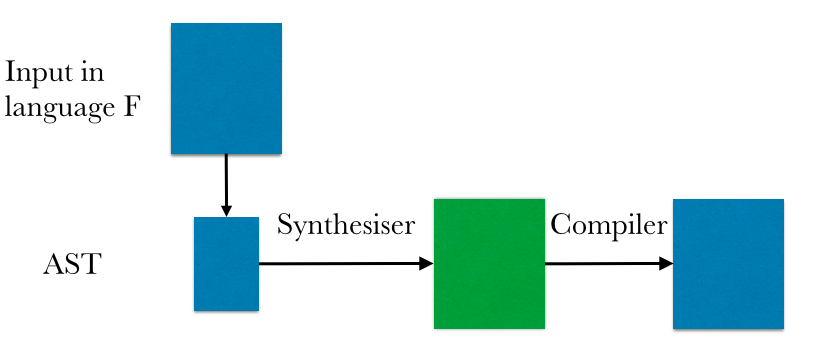
\includegraphics[width=0.8\textwidth]{images/synth.png}
  \caption{Overview of synthesiser.}
  \label{fig:synth}
\end{figure}

%------------------------------------------------------------------------------
% Evaluation
%------------------------------------------------------------------------------
\section{Evaluation}
In order to evaluate the functionality of our synthesiser we produced
a series of inputs in language $F$ to be used by the synthesiser to
generate the necessary parts of the compiler. Once we generated the
compiler we wrote a number of programs in language $F$, compiled them
using the synthesised compiler and evaluated each program using the
previously developed interpreters. If all the results were the same
then the synthesised compiler was determined to be correct. In all the
test cases the results were indeed the same. One attractive aspect of
this technique is the input programs needed to generate the compiler
are very small. 

%------------------------------------------------------------------------------
% Challenges
%------------------------------------------------------------------------------
\section{Challenges}
There were a number of challenges that had to be overcome, the first
of this was the challenges presented by using Rascal. While there are
a number of attractive features the language provides it is still in
the alpha stages and documentation can be often lacking sufficient
detail. This forced some decisions about the structure of the
languages that weren't necessarily ideal, but were the only apparent
ways to accomplish them in Rascal. This is, of course, in addition to
developing two languages with the goal of compiling one language into
the other.

The main challenge of the project was determining how to generalise
the synthesiser enough to translate nodes of language $F$ to nodes of
language $S$ without simply pattern matching each type of node and
producing the corresponding \texttt{comp} function. As the project
progressed into the final stages and some of the more complicated
transformations were attempted, it became apparent the entire method of
synthesis wasn't general enough. One possibility to generalise code
the synthesiser generates even more is to provide two inputs for each
transformation: one input in language $F$ and one input in language
$S$. The synthesiser would then analyse the input tree, from language
$F$ and synthesise code to translate nodes of that type to nodes of
the type of language $S$. This is instead of trying to figure out all
of the information from a single input in language $F$. This will also
allow us to perform more complicated transformation, such as
transformations from nodes of one type to nodes of a different type. A
concrete example of this would be to translate \texttt{let} nodes in
language $F$ to simple \texttt{app} nodes in language $S$. In the
current system this isn't possible because the synthesiser only has
the information pertaining to the tree generated for the program in
language $F$ and doesn't have any information about what that program
should be translated to. This is a fundamental flaw in the system.

%------------------------------------------------------------------------------
% Future Work
%------------------------------------------------------------------------------
\section{Future Work}
There are number of very interesting directions this project could go
from here. The first and foremost is to refine the languages to a more
reasonable form. One idea would be to use a simple core
lambda calculus as language $S$ and slightly more complicated version
for language $F$. The main focus of the future work will be to
determine a viable method for using inputs from both languages to
generate functions to compile programs from language $F$ to language
$S$. Being able to use the information from both types of programs
will greatly increase the power of the synthesiser.

In addition to this the work can move on to synthesiser more advanced
language features such as \texttt{switch} statements, \texttt{while}
loops, etc. Lastly, this type of process could be used to try
synthesising transformation on a `real' language (i.e. a language
actually used by programmers today such as Java, Javascript, etc).

\bibliography{report}{}
\bibliographystyle{plain}

\end{document}
